\documentclass[a4paper,12pt]{article}
\usepackage[utf8]{inputenc}
\usepackage[english]{babel}
\usepackage{subfigure}
\usepackage{graphicx}

% Title Page
\title{Upper limit for High mass X$\rightarrow$WW search}
\author{Piergiulio Lenzi}


\begin{document}
\maketitle

\begin{abstract}
\end{abstract}

\section{Introduction}
In this report we will study the statistical approach to the upper limit
computation for a high energy physics search for a new particle.  We will use
data from the 2015 run of the CMS experiment at the LHC and the corresponding
Monte Carlo (MC) simulations.

We will search for a new signal in the $WW\rightarrow{}2l2\nu$ final state.
This channel is also a decay channel for the Standard Model Higgs boson (H).
We will however search for an additional particle, named X in the following,
that is supposed to be heavier than H. 
We will scan a wide range of masses for X and, if we do not find a compelling
evidence for a signal, we will set an upper limit on the  cross section of X.

\section{The physics case}
In this experience we will search for the existence of a new hypothetical high
mass particle, named X. {\bf We expect this particle to be a heavy variant of
the Standard Model Higgs boson}.  For this reason we hypothesize that X shares
with H the production mechanism. This is a reasonable assumption that is
verified in several new physics models.
In particular we assumes that X can be produced via two main production
mechanisms, called gluon fusion (ggF) and vector boson fusion (VBF),
represented by the diagrams in Fig.~\ref{fig:prod}.  \begin{figure}
 \centering
 \subfigure[ggF]{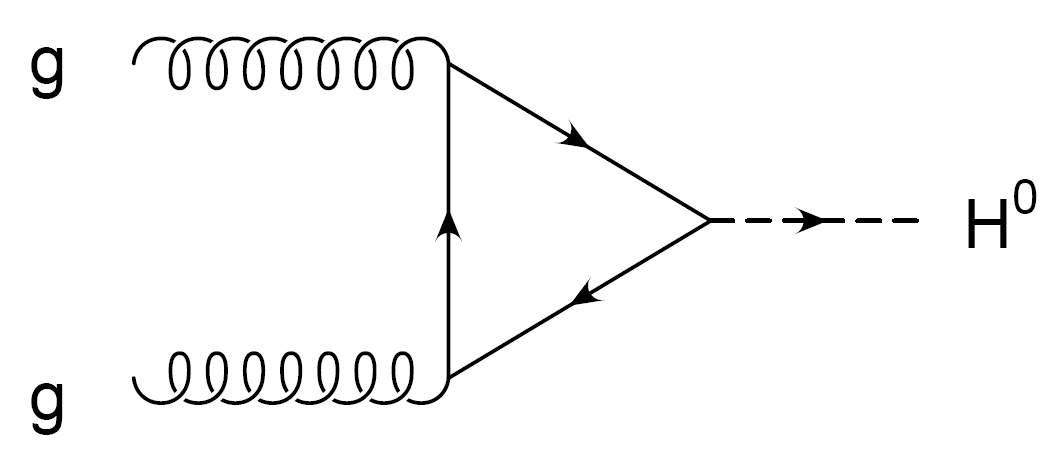
\includegraphics[width=0.4\textwidth]{images/gluon_fusion.png}}
 \subfigure[VBF]{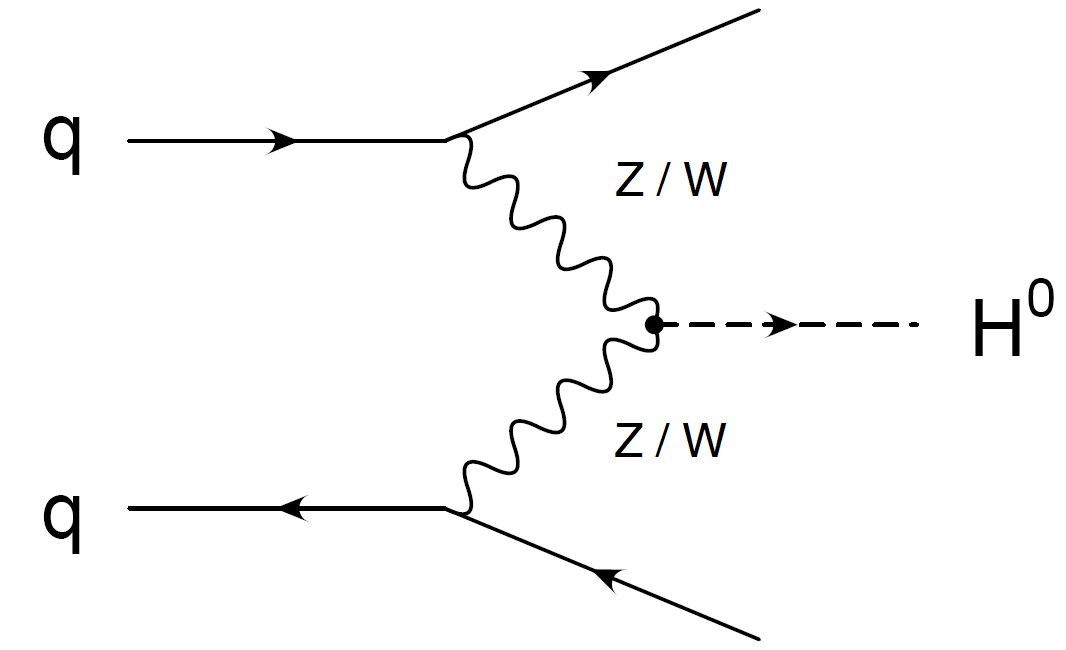
\includegraphics[width=0.3\textwidth]{images/vector_boson_fusion.png}}
 \caption{Feynmann diagrams of the two main production mechanisms for X.\label{fig:prod}}
\end{figure}

The details and precise meaning of the Feynman dagrams of Fig.~\ref{fig:prod}
are not relevant for this exercise, the relevant piece of information is that
two mechanisms are available and that they are marked by a substantial
difference: {\bf the ggF shows no other particles in the final state beyond X,
the VBF has two quarks in addition to the X in the final state}.
Although it should be noted that a precise calculation shows that additianal
particles in the form of hadronic jets can also arise in ggF, it remains true
that events arising from the two mechanisms are different when it comes to the
number of jets produced in addition to the X particle.

The production cross section for the Higgs boson as a function of its mass is
reported in Fig.~\ref{fig:production}. Although we now know the mass of the
Higgs boson to be 125 GeV, this plot is useful because it can be used as a
model for the expected cross section for X.
\begin{figure}
 \centering 
 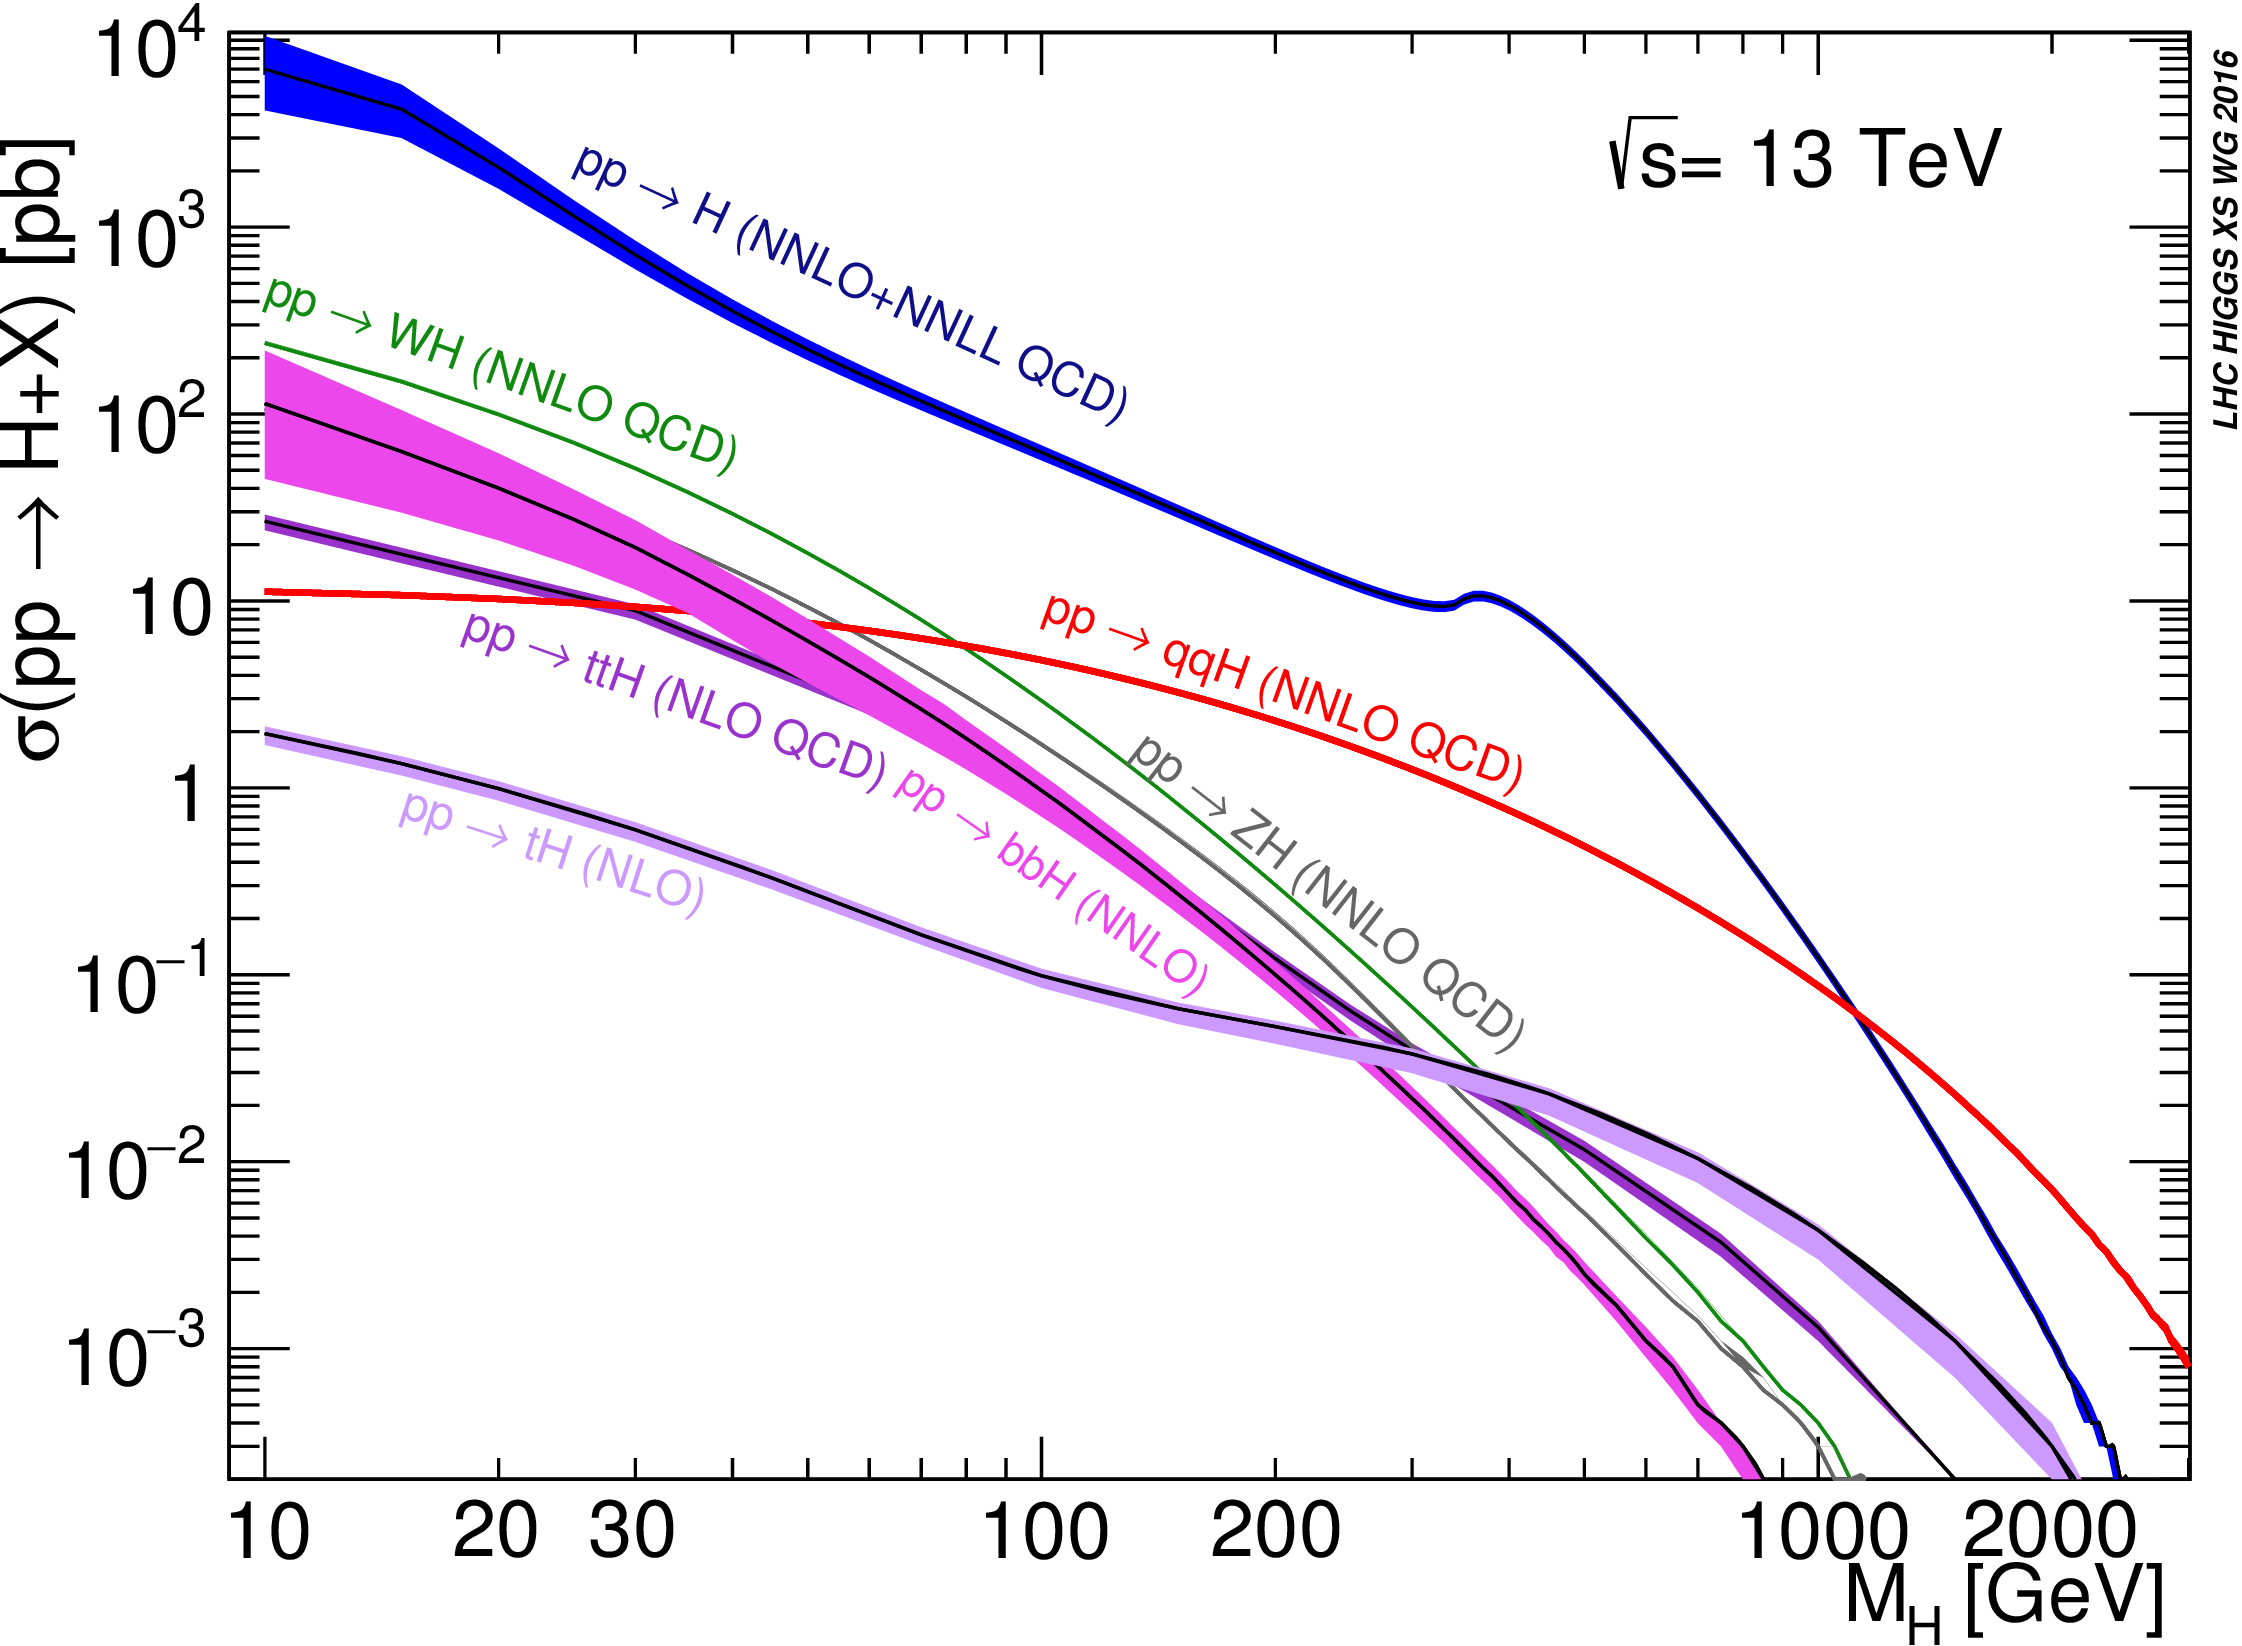
\includegraphics[width=0.5\textwidth]{images/plotAll_13tev_BSM_sqrt.png}
 \caption{Standard model Higgs boson cross section as a function of the mass
 of the Higgs boson. The ggF mechanisms is labeled $pp\rightarrow{}H$, the VBF
 mechanism is labeled $pp\rightarrow{}qqH$. Also other, sub-leading mechanisms
 are reported, which we will neglect.\label{fig:production}}
\end{figure}

We will assume that the cross section $\sigma$ for each of the production
channels of X scales with a common factor $\mu$ of the corresponding Higgs
boson cross section: 
\begin{equation}
 \sigma_{X [ggF,VBF]}(M) = \mu(M)\sigma_{H [ggF,VBF]}(M)
 \label{eq:mudef}
\end{equation}
 where M is the mass of X, and obvious meaning of the other symbols. This is a
 reasonable assumption, verified by several new physics models.  We notice
 that {\bf the relative importance of the VBF mechansm grows with the X mass},
 and becomes dominant above $\sim$1.5 TeV.
 
 We will assume that, like H, also X has several decay channels. We assume
 that X has the same branching ratios of H, which are summarized in
 Fig.~\ref{fig:br}.  \begin{figure}
 \centering 
 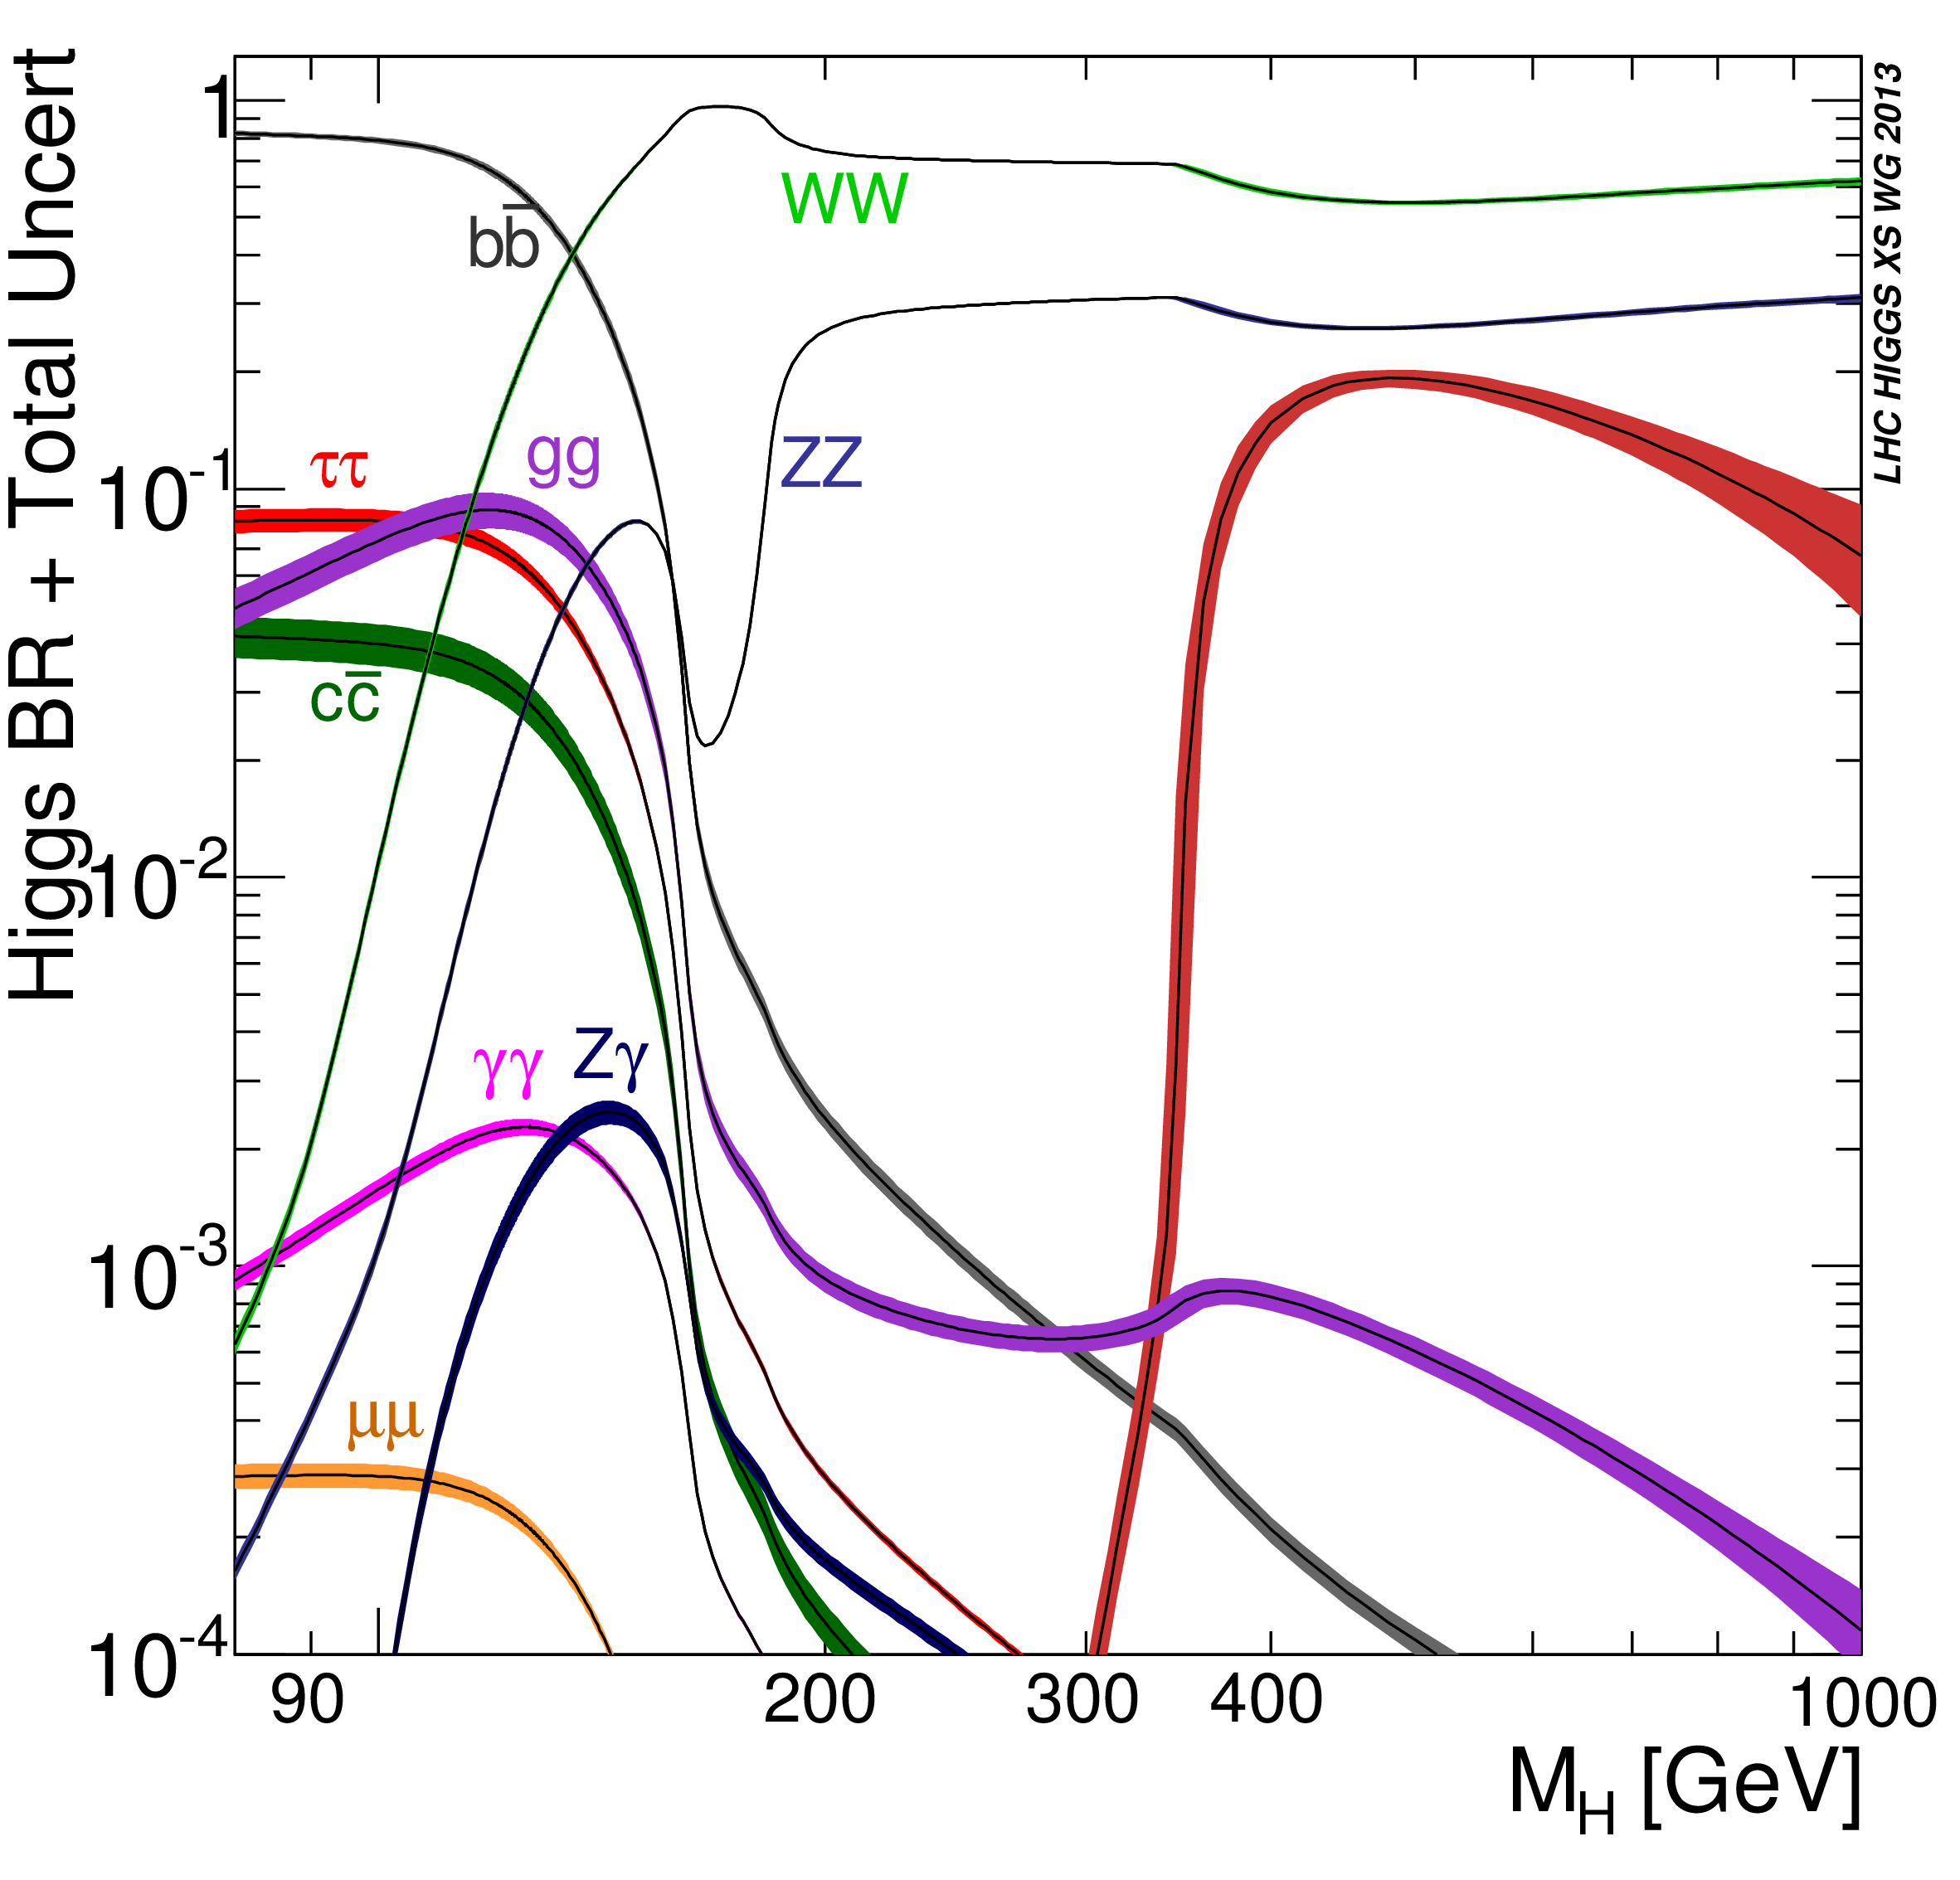
\includegraphics[width=0.5\textwidth]{images/Higgs_BR.png}
 \caption{Standard model Higgs boson cross section as a function of the mass
 of the Higgs boson. The ggF mechanisms is labeled $pp\rightarrow{}H$, the VBF
 mechanism is labeled $pp\rightarrow{}qqH$. Also other, sub-leading mechanisms
 are reported, but we will neglect them.\label{fig:br}}
\end{figure}
It should be noted that {\bf the WW decay channel is the one with the highest
branching ratio}.

\section{Data sample and analysis strategy}
Owing to the large branching fraction in the WW final state we choose this
channel for our search. In other words we search for the decay
X$\rightarrow$WW. The W bosons are themselves unstable. 30\% of the times
 a W boson decays to a charged lepton (electron, muon, tauon) and a neutrino
 (10 \% for each of the three lepton species). The remaining 70\% of the times
 the W boson decays to a pair of hadrons. In this exercise we will concentrate on the leptonic decays of the W
bosons. The reason of this choice will become clearer when we discuss
backgrounds, but let us mention already that requiring leptons in the final
state allows a dramatic reduction of background processes. 
To summarise, {\bf we search for the H$\rightarrow$WW$\rightarrow{}2l2\nu$ decay
chain}.

We will use data collected by the CMS experiment in the 2015 data taking at
the LHC. These data correspond to an integrated luminosity of 2.3~fb$^{-1}$.
We will base our analysis on data reconstructed with the official CMS software
and Simulations for both the signal and the background processes. These data
come in the form of ROOT trees.

For each event the tree stores several event variables, in particular:
\begin{itemize}
\item[-] reconstructed leptons kinematic variables;
\item[-] the reconstructed missing transverse energy;
\item[-] the reconstructed jet kinematic variables.
\item[-] several weights, used both to improve the Data/Simulation agreement
and to normalize the simulation to the data luminosity.
\end{itemize}

\subsection{Main backgrounds}
A background process in a high energy physics analysis is a physics process
that yields a final state that resembles that of the signal.
In the case of this analysis there are two main background processes:
\begin{itemize}
\item production of two W bosons without an intermediate X;
\item production of a pair of top quarks, $t\bar{t}$. The top quark decays to
a b quark and a W boson.
\end{itemize}
The Feynman diagrams of these two processes are reported in
Fig.~\ref{fig:backgrounds} for the interested reader.

\begin{figure}
\centering
\subfigure{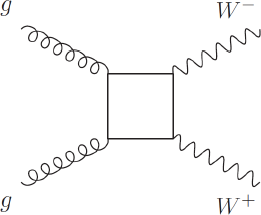
\includegraphics[width=0.3\textwidth]{images/ggWW.png}}
\subfigure{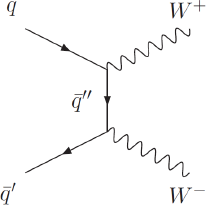
\includegraphics[width=0.3\textwidth]{images/qqWW.png}}
\subfigure{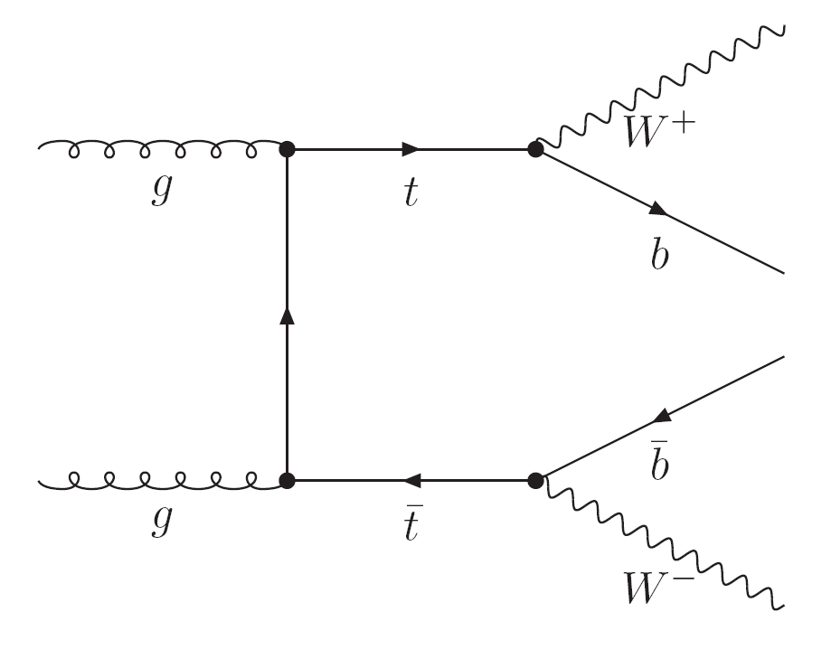
\includegraphics[width=0.3\textwidth]{images/ggtt.png}}
\caption{Gluon initiated (a) and quark initiated (b) WW. Top pair production
(c).\label{fig:backgrounds}}
\end{figure}

We apply a series of cuts to reduce their contribution as much as possible.
$t\bar{t}$ is reduced by requiring that jets in the event are not compatible
with being originated from b quarks, using dedicated jet-tagging techniques.
WW is reduced with kinematic cuts on the leptons.

Other subleading sources of background originate from processes in which at
least one of the leptons is not a real lepton, but is identified as such by the
reconstruction algorithms. The control of these backgrounds is a crucial part of the analysis,
but is beyond the scope of this exercise. The cuts to be applied will be
provided by the teachers.

\subsection{Main discriminating variable}
After the selection cuts mentioned above we end up
with a sample that is primarily composed of WW and $t\bar{t}$. In order to
further discriminate a possible signal we use a kinematic
variable called $m_{T,i}$. This variable is the invariant mass of the
4-momentum resulting from the sum of the two lepton 4-momenta and the MET
4-momentum. Since we are unable to reconstruct the longitudinal component of
the neutrinos momenta, this variable is the closest approximation of
the resonance invariant mass that we can reconstruct in a signal event, and it retains a
significant discriminating power with respect to backgrounds.

The distribution of  $m_{T,i}$ is shown in Fig.~\ref{fig:mti} after the
selection cuts. The data point are show on top of the stack of the
backgrounds. The shape of a signal for X mass of 1 TeV is also shown
(multiplied by 10). The rightmost bin of each distribution is an overflow bin.
The fact that the signal shape does not peak at 1 TeV is due to 
$m_{T,i}$ lacking the contribution from the longitudinal  momenta of neutrinos.
\begin{figure}[!b]
\centering
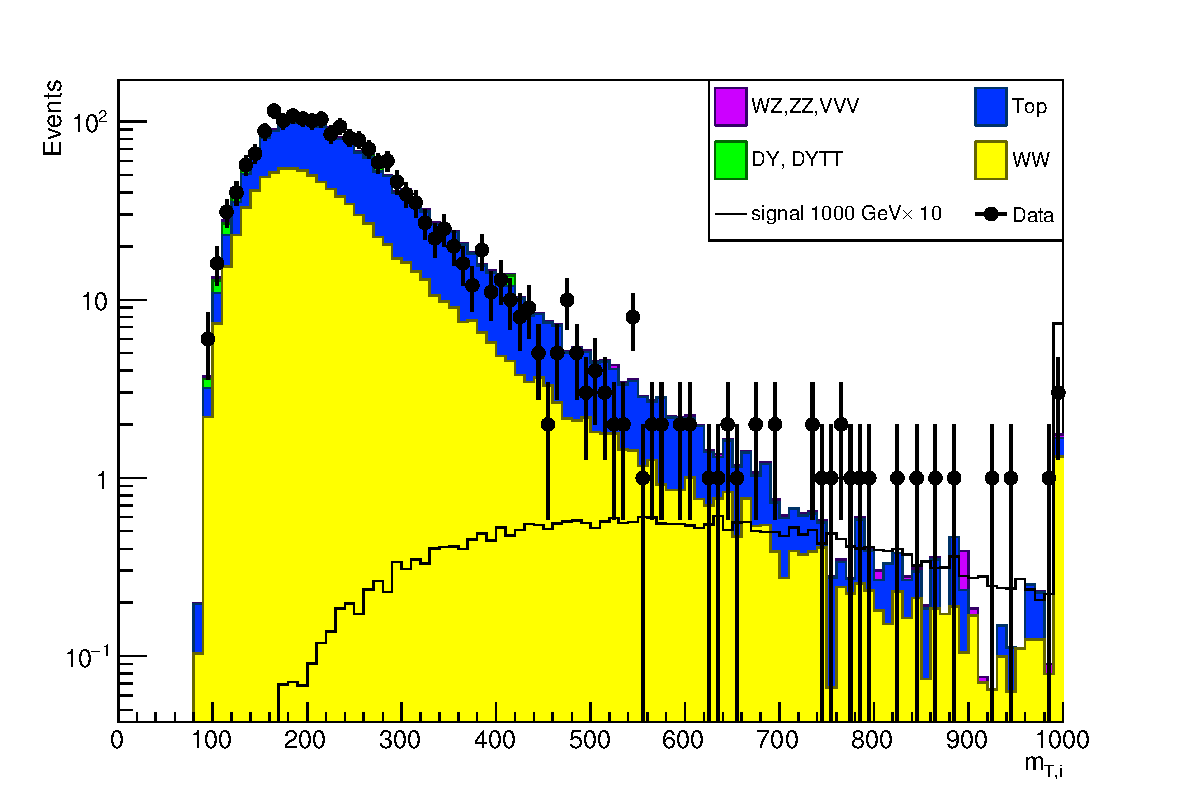
\includegraphics[width=0.6\textwidth]{images/mTi.pdf}
\caption{$m_{T,i}$ in data and simulation for 2015 data after selection cuts.\label{fig:mti}}
\end{figure}

\subsection*{Exercise 1: }
{\bf Write a code that builds the stack of backgrounds to obtain a plot
similar to Fig.~\ref{fig:mti}.}

A set of root files is provided, together with a root macro
(\verb;HWWYields.C;) implementing selection cuts.

Each root file contains a root tree named \verb;latino;. This tree holds
several variables, including $m_{T,i}$ in a branch called \verb;mTi;.

Eight data files are provided, corresponding to two distinct data taking periods
(called \verb;Run2015C; and \verb;Run2015D;) and four triggers. Data from CMS
are in fact divided into different streams depending on the triggers each
event fires. In this analysis we use events with at least two electrons
(\verb;DoubleEG;), at least two muons (\verb;DoubleMu;), at least an electron and a muon
(\verb;MuonEG;) or at least a muon  (\verb;SingleMuon;). The latter is used
only to recover an inefficiency in the other triggers.

Simulated events (MC) are produced for several physics processes, including
$t\bar{t}$, WW, Z$\rightarrow{}\tau\tau$, and other subleading processes.
Simulated samples for different mass hypotheses for X are also provided. For
each mass hypothesis two different files are provided, one containing the
simulation of the ggF production mechanism and the other containing the
simulation for the VBF production mechanism.

Simulated events are weighted with several weights that are aimed at bringing
data and MC in close agreement. We will not discuss these weight in detail. We
will just discuss an important weight contained in the branch named
\verb;baseW;. This variable is used to equalize the
luminosity of all samples to 1/fb.

Running \verb;HWWYields.C; results in a root file (\verb;yields.root;)
containing one histogram for each background, one for each signal and one for the
data. The variable plotted and the binning are controlled in the first few
lines of \verb;HWWYields.C;.

Please write a root macro that builds a stack of all the backgrounds,
superimposes the data and one signal for reference.

\subsection{Cut based analysis}
In order to check whether the data are consistent with the signal+background
hypothesis or with the background only hypothesis, we can proceed to counting
events passing our selection. Let $N_{obs}$ be the data events after the
selection, $\nu_b$ be the expected number of background evens and $\nu_s$ be
the expected number of signal events for an X signal with mass $M$. 
We expect $N_{obs}$ to follow the Poisson statistics with an average of
$\nu_b+\nu_s$ in the signal+background hypothesis and $\nu_b$ in the
background only hypothesis.

The best estimate that we can give of the number of signal events, based on a
single experiment, is
\begin{equation}
\hat{\nu}_s=N_{obs}-\nu_b
\label{eq:nuhat}
\end{equation}
where the dependency on the mass hypothesis is there to remind us that the
analysis cuts can be different depending on the mass of the signal we search
for.

In order to understand whether the obtained value of $\hat{\nu}_s$ is
significantly different from 0 we should compare it with the statistical
fluctuation of the expected background. Only if $\hat{\nu}_s$ is larger
than several standard deviations (5) of the expected background we can claim a
discovery.

Following this discussion we are left with an open question: should we ad any
other selection cuts to our selection to improve the analysis sensitivity to a
signal?

\section*{Exercise 2}
{\bf For each X mass hypothesis find the cut on $m_{T,i}$ which maximises the
sensitivity}

Fig.~\ref{fig:mti} shows that $m_{T,i}$ has a good discriminating power. In
particular if we only count events above a certain optimal value of  $m_{T,i}$ we
should be able to improve the sensitivity to a signal. 

The student should find, for each X mass hypothesis, the value of $m_{T,i}$
($m_{T,i}^{cut}$) such that by integrating events with
$m_{T,i}>m_{T,i}^{cut}$ the ratio of expected number of signal events
$\nu_s$ and the statistical fluctuation of background events
$\sqrt{\nu_b}$ ($\nu_s/\sqrt{\nu_b}$) is maximised.

\section{Upper limit with approximate formulae}
Upon completion of Exercise 2 the student has found the optimal value in
$m_{T,i}$ where one should cup in order to find a possible signal. The optimal
position of the cut depends on the mass of the hypothesized signal.

We now aim at finding the upper limit for each mass hypothesis.
We refer to Cowan's book equation 9.39. The upper limit at 95\% confidence
level on the number of signal events ($\nu_{up}$) can be found as:
\begin{equation}
\nu_{up} = \hat{\nu}_s + \delta_{\hat{\nu}_s}\cdot\Phi^{-1}(0.95)
\label{eq:limitcowan}
\end{equation}
where $\hat{\nu}_s$ is given by Eq.~\ref{eq:nuhat}, $\delta_{\hat{\nu}_s}$ 
is the error on $\hat{\nu}_s$, $\Phi^{-1}$ is the inverse cumulative distribution 
of the Gaussian.

Eq.~\ref{eq:limitcowan} {\bf holds under the assumption that the distribution of
$\hat{\nu}_s$ is Gaussian}. However $\hat{\nu}_s$, as defined in
Eg.~\ref{eq:nuhat} comes as the difference between a random variable
distributed according to Poisson distribution ($N_{obs}$) and a number. The
assumption that $\hat{\nu}_s$ is Gaussian is only valid in case $N_{obs}$
has a relatively large expectation value, so that the difference between
Poisson and Gaussian distribution can be neglected.

How do we estimate $\delta_{\hat{\nu}_s}$? If we know the number of
expected background events with no error, then
$\delta_{\hat{\nu}_s}=\sqrt{N_{obs}}$, following Poisson statistics. 

However we usually have an uncertainty on the estimation of the number of
background events $\delta_{\nu_b}$. This kind of uncertainty is systematic, contrary to the
uncertainty on $N_{obs}$, which is statistical instead. It is not obvious how
to combine the two uncertainties into $\delta_{\hat{\nu}_s}$.

In the following we will make a common choice, which consists in combining the
two uncertainties as one would do if they were both statistical. It then
follows that
\begin{equation}
\delta_{\hat{\nu}_s}=\sqrt{N_{obs}+\delta_{\nu_b}^{2}}.
\label{eq:errorCinghiale}
\end{equation}
Let us discuss in some more detail the meaning of our choice of summing in
quadrature the genuinely statistical uncertainty on $N_{obs}$ and the
systematic uncertainty $\delta_{\nu_b}$.
By doing this we are effectively expressing our degree of belief in our
estimate of the background in the form of a Gaussian with average $\nu_b$ and
standard deviation $\delta_{\nu_b}$. Indeed, if you assume that the true value
of the expected number of background events is distributed as a Gaussian of
standard deviation $\delta_{\nu_b}$ around the average $\nu_b$, then the
variance of $\hat{\nu}_s$ is indeed given by Eq.~\ref{eq:errorCinghiale}.

In other words we are weighting the probability that we are wrong about our
estimate of the number of background events in a Gaussian way
with respect to our best estimate $\delta_{\nu_b}$. It should be somewhat clear from the choice of words in
the two past sentences that we are to some extent entering the realm of
Bayesian probability, in that we are using a PDF, a Gaussian in this case, to
measure how sure we are of our background estimate.

It should be clear that using a Gaussian to describe our degree of belief in
the background estimate, as an effective way of modeling the systematic
uncertainties is not the only option. Other systematic uncertainties may be
better modeled by different PDFs, such as Uniform, of lognormal. It is in
general a good practice (although not always done in practice) to test the
robustness of a result against the (somewhat arbitrary) choice of the PDF that
models the systematic uncertainties.

\section*{Exercise 3}
{\bf Derive an upper limit on the signal strength $\mu$ using
Eq.~\ref{eq:limitcowan}}

Using the signal and background yields obtained from the mass dependent cuts
of Exercise 2, the student should plot the expected and observed limit.

The systematic uncertainty on the background should be taken to be a
(reasonable) 10\% of $\nu_b$.

The {\bf expected limit is the limit you expect to put in the background
only hypothesis}. It can be derived very simply by assuming $\hat{\nu}_s$=0.
This however does not give you any sense of how the statistical fluctuations
in the number of observed events may affect the limit. 

In order to have such an idea the student should make several
``toy'' experiment, i.e. they should simulate what the result of an
experiment  could be in a background only hypothesis. In our simple case this
boils down to throwing several random numbers according to the Poisson
distribution around $\nu_b$. Each random extraction $i$ would yield a number
$N_{obs}^i$. For each $N_{obs}^i$ the student should compute the upper limit
according to Eq.~\ref{eq:limitcowan}. The expected limit can be extracted by
taking the median of the limits obtained in all the toy extractions. Similarly
a 1 and 2 sigma band can be extracted by taking the 2.5\% percentile
(2$\sigma$ down), 34\% (1$\sigma$ down), 84\% (1$\sigma$ up), 97.5\%
(2$\sigma$ up) of the distribution of expected limits from toys for each mass. 

The observed limit is the limit obtained from data, using $N_{obs}$ from data.
The student should finally obtain a plot similar to the one shown in
Fig.~\ref{fig:limitCowan}.
\begin{figure}[!b]
\centering
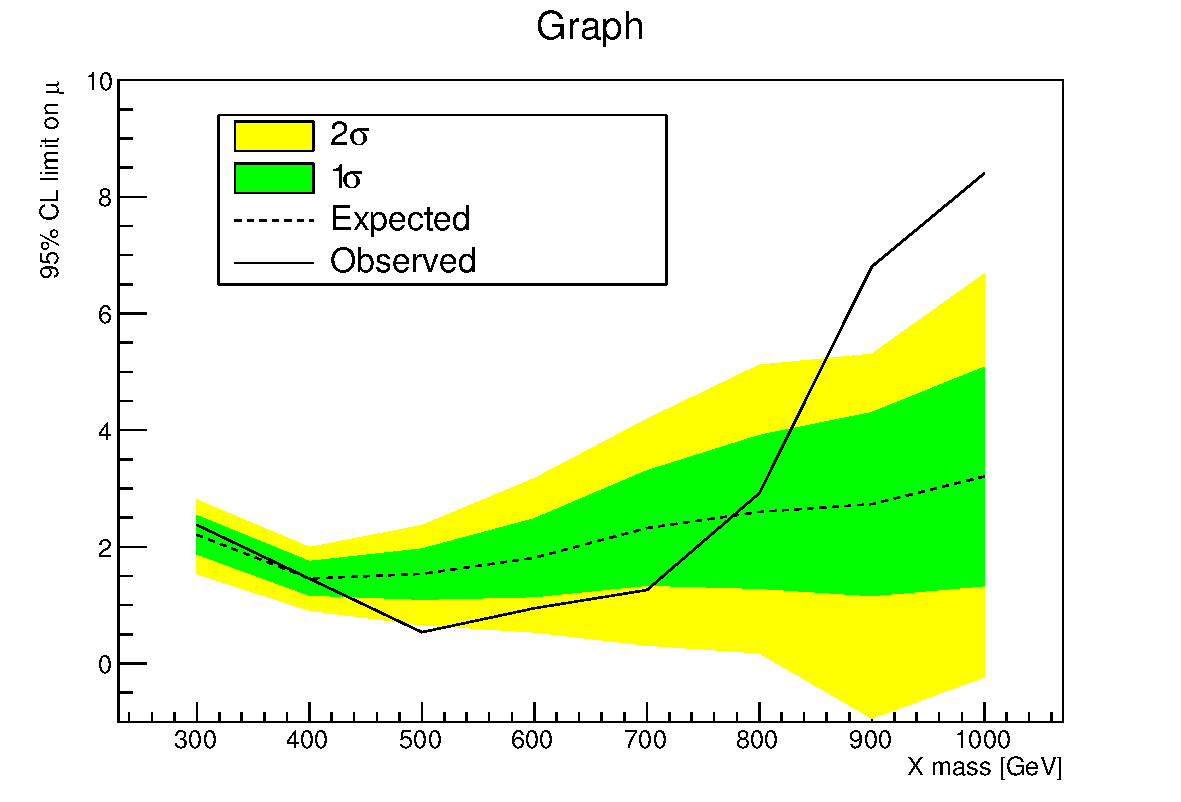
\includegraphics[width=0.5\textwidth]{images/limitCowan.pdf}
\caption{Expected and observed limit. The result of Exercise 3 should be
something of this form.\label{fig:limitCowan}}
\end{figure}

\section{Maximum likelihood estimator of the signal strength}
In this paragraph we will introduce the maximum likelihood fit as a way to
estimate the signal strength in the presence of systematic uncertainties.
We spell out since the beginning that the systematic uncertainties will be
included in the fitting procedure in the form of parameters for which an external
constraint is imposed in the fit. Parameters in a maximum likelihood fit which
represent systematic uncertainties are called {\bf nuisance parameters}, to
distinguish them from the parameters for which we do not put external
constraints, such as the signal strength ($\mu$) in our case, which are known as {\bf
parameters of interest (POI)}. 

Let us assume that the random variable that we measure in our experiment is
$N_{obs}$. We expect it to be Poisson-like distributed around
$\nu_b+\mu\cdot\nu_s$, where $\nu_s$ is the number of signal events we expect
for the signal, if X is actually the SM H (remember Eq.~\ref{eq:mudef}).
In this case the likelihood function $\mathcal{L}(\mu)$ is simply:
\begin{equation}
\mathcal{L}(\mu)=\frac{(\nu_b+\mu\cdot\nu_s)^{N_{obs}}}{N_{obs}!}e^{-(\nu_b+\mu\cdot\nu_s)}
\label{eq:likelihood_no_nuisances}
\end{equation}
Maximizing $\mathcal{L}(\mu)$ with respect to $\mu$ gives the best fit value
for $\mu$, $\hat{\mu}$. The result is the already known result of Eq~\ref{eq:nuhat}, 
which we can express in terms of $\mu$ as
\begin{equation}
\hat{\mu} = \frac{N_{obs}-\nu_b}{\nu_s}.
\end{equation}

We can introduce our degree of belief in the knowledge of the background
distribution in the form of a nuisance parameter with an external constraint
in the likelihood $\mathcal{L}(\mu)$. Let us for example assume that we know
the normalization of the background with a relative uncertainty
$\delta_{\nu_b}/\nu_b$, and let us introduce the nuisance parameter $\mu_b$,
which is a multiplier of $\nu_b$ in much the same way as $\mu$ is multiplier for the
number of expected signal events. 

In order to add a constraint on $\mu_b$ in the likelihood we simply have to
multiply the likelihood of Eq.~\ref{eq:likelihood_no_nuisances} by a Gaussian
constraint on $\mu_b$ with standard deviation $\delta_{\nu_b}/\nu_b$. The new
likelihood function is now function of both $\mu$ (the POI) and $\mu_b$ (a
nuisance parameter), and reads:
\begin{equation}
\mathcal{L}(\mu;\mu_b)=\frac{1}{2\pi\frac{\delta_{\nu_b}}{\nu_b}}e^{-\frac{(\mu_b-1)^2}{2(\frac{\delta_{\nu_b}}{\nu_b})^2}}\times\frac{(\mu_b\cdot\nu_b+\mu\cdot\nu_s)^{N_{obs}}}{N_{obs}!}e^{-(\mu_b\cdot\nu_b+\mu\cdot\nu_s)},
\label{eq:likelihood_nuisance}
\end{equation}
where the initial part before the $\times$ symbol is the Gaussian constraint
on $\mu_b$.

The reader might be surprised by the fact that by maximizing
Eq.~\ref{eq:likelihood_nuisance} we are effectively fitting two parameters
(the POI $\mu$ and the nuisance $\mu_b$) with a single measurement
($N_{obs}$). One should remember, however, that the second constraint effectively comes from the assumed shape of
the distribution of the nuisance parameter, a Gaussian in this case.

The likelihood function of Eq.~\ref{eq:likelihood_nuisance} can be easily
extended to the case in which our measurement consists of a vector of
$n$ random variables $\vec{N}_{obs}=(N_{obs}^1...N_{obs}^n)$. We would like to draw the
reader's attention on the fact that this is exactly the case we have when we measure number
of events in a binned histograms with $n$ bins, such as in
Fig.~\ref{fig:mti}. To extend Eq.~\ref{eq:likelihood_nuisance} to handle this
case, one simply needs to introduce a product of Poisson distributions, one
for each of the $n$ bin. 

Similarly Eq.~\ref{eq:likelihood_nuisance} can be easily
extended to the case in which we have more nuisances. For example, our
background could be (and most likely will be) composed by several contributions (e.g. one for each different
background process), each with their own normalization uncertainty. In this case one simply add each nuisance as a
multiplicative constraint in the likelihood. Also, the functional form of each constraint could
be different for the different constraints.

Although the formalism introduced in this paragraph might sound like an
overkill for a simple measurement counting experiment such as the one we are
considering in this experiment, this formalism allows for handling of
arbitrary number of bins and arbitrary number of nuisances. Consider for
example that the H$\rightarrow{}$WW analysis in CMS has around 100 bins, a  variable number of
POIs, ranging from 1 to 10 depending on the particular quantity that is
measured, and
several tens of nuisance parameters.



\end{document}          
